% vim: set textwidth=78 autoindent:

\subsection{Complemento Oracle GeoRaster}

% when the revision of a section has been finalized, 
% comment out the following line:
% \updatedisclaimer

En bases de datos Oracle, los datos raster pueden ser almacenados en objetos SDO\_GEORASTER disponibles con la extensión Oracle Spatial. En QGIS, el \toolbtntwo{oracle_raster}{Complemento Oracle GeoRaster} 
es soportado por GDAL, y depende del producto de Bases de Datos Oracle instalado y trabajando en tu máquina. Mientras Oracle es software propietario, ellos proveen su software gratis para propósitos de desarrollo y pruebas. Aquí está un ejemplo simple de como cargar imágenes raster a GeoRaster:

\begin{verbatim} 
$ gdal_translate -of georaster input_file.tif geor:scott/tiger@orcl
\end{verbatim}

Esto cargará el raster dentro de la tabla predeterminada GDAL\_IMPORT, como una columna llamada RASTER.

\subsubsection{Administrando conexiones}

Primeramente, el complemento Oracle GeoRaster debe estar activado usando el Administrador de complementos (vea la sección 
\ref{sec:load_core_plugin}). La primer vez que carga un GeoRaster en QGIS, debe crear una conexión 
a la base de datos de Oracle que contiene los datos. Para hacer esto, comience haciendo clic en 
el botón de la barra de herramientas \toolbtntwo{oracle_raster}{Seleccionar GeoRaster}, abrirá el diálogo Seleccionar GeoRaster Espacial. Clic en \button{Nuevo} para abrir el diálogo, y especificar los parámetros 
de conexión (vea la figura \ref{fig:oracle_create}):

\begin{itemize}
\item \textbf{Nombre}: Escriba un nombre para la conexión de base de datos.
\item \textbf{Instancia de la base de datos}: Escriba el nombre de la base de datos a la que se conectará.
\item \textbf{Nombre de usuario}: Especifique el nombre de usuario que usará para accesar a la base de datos.
\item \textbf{Contraseña}: La contraseña asociada con el nombre de usuario requerido para accesar la base de datos.
\end{itemize}

\begin{figure}[ht]
   \begin{center}
   \caption{Diálogo crear conexión a Oracle \nixcaption}\label{fig:oracle_create}\smallskip
   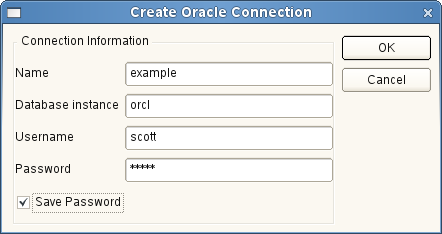
\includegraphics[clip=true, width=9cm]{oracle_create_dialog}
\end{center}
\end{figure}

Ahora, de regreso en el diálogo principal de Oracle GeoRaster espacial (vea la figura \ref{fig:oracle_select}), use la lista desplegable para elegir una conexión, y use el  
botón \button{Connectar} para establecer una conexión. Puede también 
\button{Editar} la conexión abriendo el diálogo previo y haciendo cambios a la información de conexión, o use el botón \button{Eliminar} para remover la conexión desde la lista desplegable.

\subsubsection{Seleccionando un GeoRaster}

Una vez que la conexión ha sido establecida, la ventana de subconjuntos de datos mostrará los nombres de todas las tablas que contiene columnas GeoRaster en la base de datos en el formato de un nombre de subconjunto de datos de GDAL.

Haga clic en uno de los subconjuntos listados y entonces clic en \button{Seleccionar} para elegir el nombre de tabla. Ahora otra lista de subconjuntos de datos se mostrará con los nombres de columnas GeoRaster en esa tabla. Esta es usualmente una lista pequeña, ya que la mayoría de los usuarios no tendrán mas de una o dos columnas GeoRaster en la misma tabla.

Haga clic en uno de los subconjuntos listados y entonces clic en el botón \button{Seleccionar} para elegir una de la combinación tabla/columna. El diálogo ahora mostrará todas las filas que contienen objetos GeoRaster. Note que la lista de subconjuntos de datos ahora mostrará pares de la tabla de datos raster   e ids raster.

En cualquier momento la entrada de la selección puede ser editada para ir directamente a un GeoRaster conocido o ir al inicio y seleccionar otra tabla.

\begin{figure}[ht]
   \begin{center}
   \caption{Diálogo seleccionar Oracle GeoRaster \nixcaption}\label{fig:oracle_select}\smallskip
   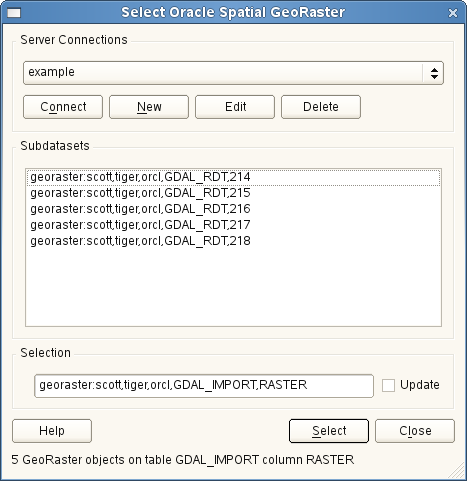
\includegraphics[clip=true, width=9cm]{oracle_select_dialog}
\end{center}
\end{figure}

La selección de datos de entrada puede también ser usada para escribir clausulas Where al final de la cadena de identificación, ej., 
``geor:scott/tiger@orcl,gdal\_import,raster,geoid=''. vea \url{http://www.gdal.org/frmt_georaster.html} para mas información.

\subsubsection{Mostrando GeoRaster}

Finalmente, seleccionando un GeoRaster de la lista de Tablas de Datos Raster e Ids Raster, la imagen raster será cargada a QGIS.

El diálogo seleccionar Oracle GeoRaster Espacial puede ser cerrado ahora y la siguiente vez que la abra mantendrá la misma conexión, y mostrará la misma lista previa de subconjuntos de datos haciendo muy fácil abrir otra imagen del mismo contexto.

\textbf{Nota:} GeoRasters que contienen pirámides se mostrarán mucho mas rápido pero las pirámides necesitan ser generadas fuera de QGIS usando Oracle PL/SQL o gdaladdo.

El siguiente es un ejemplo usando gdaladdo:

\begin{verbatim}
gdaladdo georaster:scott/tiger@orcl,georaster\_table,georaster,georid=6 -r 
nearest 2 4 6 8 16 32
\end{verbatim}

Este es un ejemplo usando PL/SQL: 
cd ..
\begin{verbatim}
$ sqlplus scott/tiger
SQL> DECLARE
    gr sdo_georaster;
BEGIN
    SELECT image INTO gr FROM cities WHERE id = 1 FOR UPDATE;
    sdo_geor.generatePyramid(gr, 'rLevel=5, resampling=NN');
    UPDATE cities SET image = gr WHERE id = 1;
    COMMIT;
END;
/
\end{verbatim}

